\documentclass[USenglish,pdftex,compress,10pt,svgnamesi,handout]{beamer}
%\documentclass[USenglish,pdftex,compress,10pt,svgnamesi]{beamer}%


\usepackage{tikz}
\usetikzlibrary{positioning}
\usetikzlibrary{bayesnet}

\usefonttheme[onlymath]{serif}
\usepackage[ansinew]{inputenc}      % direkte Eingabe von Umlauten
\usepackage{graphicx}   % picture inclusion
\usepackage{amsmath}    % extended math stuff
\usepackage{amsfonts}   % corresponding fonts
\usepackage{bm}         % improved Greek bold math

\usepackage[english]{babel}

\usepackage[square]{natbib}  % reference 
\usepackage{booktabs}
\usepackage{ae}          % PDF-compatible fonts

\setbeamertemplate{footline}[frame number]

\newcommand{\imgcrop}[4]{  % filename, title, boxwidth, viewport
\centering\begin{beamerboxesrounded}[upper=fig,lower=block body,width=#3,shadow=true]{#2}
\includegraphics[width=\textwidth,viewport=#4]{pics/#1}
\end{beamerboxesrounded}
}
\newcommand{\imgbox}[3]{   % filename, title, boxwidth
\centering\begin{beamerboxesrounded}[upper=fig,lower=block body,width=#3,shadow=true]{#2}
\includegraphics[width=\textwidth]{pics/#1}
\end{beamerboxesrounded}
}

\newenvironment{poll}
{\begin{frame}<handout:0>
\frametitle{poll}
	\color[rgb]{0,.3,0}}
{\end{frame}}


\usetheme{Boadilla}
\usecolortheme[rgb={0,0.4,0}]{structure}
  \setbeamertemplate{enumerate items}[square]
  \setbeamertemplate{itemize items}[square]

\author{Patrick van der Smagt}
\hypersetup{%
	pdfauthor={Patrick van der Smagt}%
}


\def\target{z}


%\newcommand{\be}{\begin{equation}}
%\newcommand{\bel}[1]{\begin{equation}\label{#1}}
%\newcommand{\ee}{\end{equation}}
\newcommand*\abs[1]{\left\lvert#1\right\rvert}      % absolute value
\newcommand*\avg[1]{\left<#1\right>}                % average
\newcommand*\C{\mathcal{C}}                         % class C (for classification)

\let\orid=\d %for lower dot accent use \orid now
\renewcommand*\d[3][]{                              % differetial quotient
  \def\next{#1}%
  \ifx\empty\next
    \frac{\text{d}#2}{\text{d} #3}
  \else
    \frac{{\text{d}#2}^{#1}}{\text{d}^{#1} #3}
  \fi}
\newcommand*\D[3][]{                                % partial derivative
  \def\next{#1}%
  \ifx\empty\next
    \frac{\partial#2}{\partial #3}
  \else
    \frac{{\partial#2}^{#1}}{\partial^{#1} #3}
  \fi}
\newcommand{\Def}[1]{\alert{#1}}                    % first occurrence of a new term
\newcommand{\Annot}[1]{\qquad\text{#1}}             % annotation in (short) equation
\newcommand{\Set}[1]{\mathcal{#1}}                  % mathematical set
\newcommand*\Det[1]{\left\lvert#1\right\rvert}      % determinant
\newcommand*\diff{\text{d}}                         % differential
\newcommand*\DX{\,\text{d}x}                         % differential dx
\newcommand*\DY{\,\text{d}y}                         % differential dy
\newcommand*\E{\mathbb{E}}  % expectation value
\renewcommand*\H{\mathrm{H}}                          % Entropy
\newcommand*\KL{\mathrm{KL}}                        % Kullback-Leibler divergence
\newcommand\imagi{\text{i}}                         % \sqrt{-1} == \imagi (imaginary)
\newcommand*\Mtx[1]{\bm{{#1}}}                      % matrix quantity
\newcommand{\Norm}[1]{\lVert#1\rVert}               % norm of a matrix or vector
\newcommand*\N{\mathcal{N}}                         % Normal distribution
\newcommand*\Nset{\mathbb{N}}                       % set of natural numbers
\newcommand\Order[1]{\mathcal{O}(#1)}               % order operator
\newcommand\nate{\text{e}}                          % base of ln == \exp (natural e)
\newcommand*\Operator[1]{\mathcal{#1}}              % operator quantity
\newcommand{\ParBeg}[1]{\structure{#1}}             % new paragraph, similar to description
\newcommand*\Q{\mathbb{Q}}                          % set Q {rational numbers}
\newcommand*\R{\mathbb{R}}                          % set R {real numbers}
\newcommand*\T{^{\text{T}}}                         % transpose
\newcommand*\Tensor[1]{\bm{\mathsf{#1}}}            % tensor quantity
\newcommand{\var}{\text{var}}
\renewcommand*\Vec[1]{\bm{{#1}}}                    % vector quantity

\newcommand*\Z{\mathbb{Z}}                          % set Z {... -1, 0, 1, ...}

\newcommand{\mub}{\Vec{\mu}}
\DeclareMathOperator*{\argmax}{arg\,max}
\DeclareMathOperator*{\argmin}{arg\,min}
\newcommand*\F{\mathcal{F}}
\newcommand{\ra}[1]{\renewcommand{\arraystretch}{#1}}

\newcommand\keyword[1]{\textbf{$\rightarrow$ #1}}



\def\function{f}
\def\model{\hat\function}


\graphicspath{{pics/}}
\usepackage{picinpar}
\usepackage{color}
\usepackage{soul}
\usepackage{cancel}

\parskip2ex

\def\Vec#1{\textbf{#1}}
\def\bfx{{\Vec x}}
\def\bfw{{\Vec w}}
\def\cl#1{{\cal #1}}
\newcommand{\scalar}[2]{#1^T#2}
\newcommand{\scalarold}[2]{\left<#1,#2\right>}

\newcommand{\eq}[1]{\begin{align*}#1\end{align*}}
\newcommand\numberthis{\addtocounter{equation}{1}\tag{\theequation}}
\newcommand{\expc}{\mathbb{E}}
\newcommand{\vari}{\operatorname{Var}}
\newcommand{\covari}[2]{\operatorname{Cov}[#1,#2]}
\newcommand{\pd}[2]{\frac{\partial{#1}}{\partial{#2}}}

\newcommand{\exmpl}[1]{\par{\textbf{Example:}} #1}
\newcommand{\question}[1]{\par{\textbf{Question:}} #1}
\newcommand{\answer}[1]{\par{\textcolor{red}{\textbf{Answer:}}} #1}




% =====================================================================
% Titel etc.
\hypersetup{pdftitle={Probability Theory}}

\title{Probability Theory}
\date{July 2017}
% =====================================================================
\begin{document}

%'''''''''''''''''''''''''''''''''''''''''''''''''''''''''
\begin{frame}
	\titlepage
	
	slides almost completely by Justin Bayer

\end{frame}

\begin{frame}
\frametitle{Some random events}
\begin{columns}[t]
\column{5cm}


\includegraphics[width=\linewidth]{pics/matchpoint}

\vspace{1em}


\includegraphics[width=\linewidth]{pics/stocks}

\column{5cm}

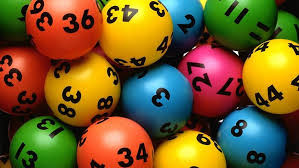
\includegraphics[width=\linewidth]{pics/lotto}

\vspace{1em}


\includegraphics[width=.5\linewidth]{pics/oldshatterhand}
\end{columns}
\end{frame}


\begin{frame}
\frametitle{Why Probability theory?}

Different things have different inherent certainties, i.e. \emph{entropy}:
\begin{itemize}
    \item We cannot really say whether a tennis ball hitting the net on top goes to right or left---unless we have a \emph{very sophisticated} physical model.
    \item We cannot predict Lotto at all, since the process is random by design.
    \item The stock market seems to correlate with all kinds of things.
    \item Old Shatterhand never misses. Or does he?
\end{itemize}
\end{frame}


\begin{frame}
\frametitle{Why Probability theory?}
\begin{itemize}
    \item If the universe were deterministic, would we need probabilities?
    \pause
    \item Yes, because we do not know everything.
    \pause
    \item We need probability to express our \emph{subjective uncertainty} about something.
\end{itemize}
\pause
\center Probability = boolean logic + uncertainty
\end{frame}


\begin{frame}
\begin{flushright}{``\it 
The probability of an event is simply a fraction whose numerator is the number of favourable cases and whose denominator is the number of all the cases possible.''
}
\\ \medskip
Pierre-Simon Laplace
\end{flushright}

Probability theory really comes down to counting. But counting can be hard.

\end{frame}


% =====================


\begin{frame}
\frametitle{Events and Random Variables 1}
Consider a box with balls. 
Each ball has a number from $1 \dots 10$ written on it.
We draw a single ball.

\medskip

Each ball corresponds to an \emph{event}.
We can design \emph{random variables} based on that event; each random variable is a \emph{function} of the event space.

\bigskip
\pause
Some examples. The number on the ball is
\begin{enumerate}
    \item odd,
    \item a prime number,
    \item greater than 12,
    \item less than 3.
\end{enumerate}
These are all \emph{indicator variables}, i.e.\ they are either \emph{true} or \emph{false}. That is statisticianlish for \emph{binary}.
\end{frame}


\begin{frame}
\center
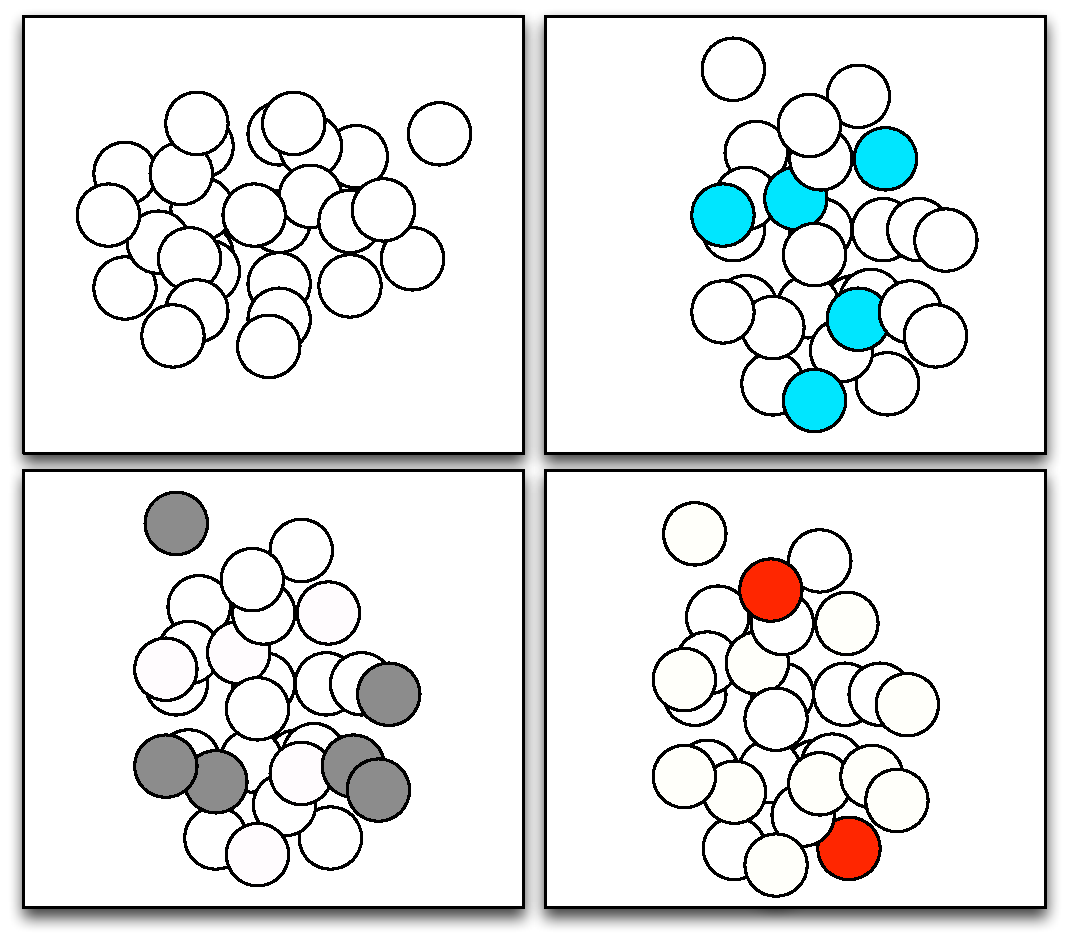
\includegraphics[width=.8\linewidth]{pics/balls}
\end{frame}


\begin{frame}
\frametitle{Events and Random Variables 2}

We can also directly retrieve the number with a random variable:

\eq{
    n: \Omega \rightarrow \{1, 2, 3, 4, 5, 6, 7, 8, 9, 10\}
}

$\Omega$ is the set of events, i.e.\ the set of all balls.
\end{frame}


\begin{frame}
\frametitle{Probabilities are fractions}
Informal:
\eq{
    p(\text{``number on ball is odd''}) 
        = \frac{\#\text{odd balls}}{\#\text{all balls}}
}
\pause
\medskip
Formal: 

Let $\omega \in \Omega$. 
Then the probability of the outcome of some indicator random variable $F: \Omega \rightarrow \{0, 1\}$ is 
$$
    p(F=1) = \frac{|\{\omega \in \Omega: F(\omega) = 1\}|}{|\Omega|}
$$

\pause
\medskip
More general:
$$
    p(F=f) = \frac{|\{\omega \in \Omega: F(\omega) = f\}|}{|\Omega|}
$$
\end{frame}


\begin{frame}
\frametitle{More than one random variable}
Let us consider two draws from the box and call the random variables $n_0$ and $n_1$.

\medskip

\question{Does it make a difference for the second ball if we put the first one back after looking at it?}
\pause
\answer{Yes, because the distribution in the box is changed.}

\question{Under what circumstances would it not make a difference?}
\pause
\answer{If there were so many balls in the box, that one missing has only a very small effect. I.e., infinitely many.}
\end{frame}


\begin{frame}
\frametitle{Joint probability}
We can also calculate the probability of two random variables taking certain values simultaneously:
\eq{p(F_0=f_0, F_1=f_1)}
\exmpl{Probability that a number on a ball is odd and divisible by 3.}
These random variables can highly influence each other!
\end{frame}

\begin{frame}
\frametitle{Conditional probability}
Consider we have already observed that a ball is odd.
What is the probability that it is divisible by 3?
\eq{p(F_0=f_0\mid F_1=f_1)}
\end{frame}


\begin{frame}
\frametitle{Marginal probability}
Consider we have modelled the world in terms of $F_0$ and $F_1$.
Then only considering one of them is called the \emph{marginal probability}:
\eq{p(F_1=f_1)}
\end{frame}


\begin{frame}
\frametitle{The most important slide of this set}
\begin{block}{Sum rule}
\eq{
    p(X) = \sum_Y p(X, Y)
}
\end{block}

\begin{block}{Product rule}
\eq{
    p(X, Y) = p(X\mid Y)p(Y)
}
\end{block}

\begin{block}{Bayes' theorem}
\eq{
    p(X\mid Y) &= \frac{p(Y\mid X)p(X)}{p(Y)}
}
\end{block}
\end{frame}


\begin{frame}
\frametitle{Independence}
Two random variables are \emph{independent} if they do not influence their respective outcomes.
\eq{
    p(X\mid Y) &= p(X)  \Rightarrow  \\
    p(X, Y) &= p(X)p(Y) \Rightarrow \\
    p(Y\mid X) &= p(Y)
}
But beware!
\medskip

\pause
{\center
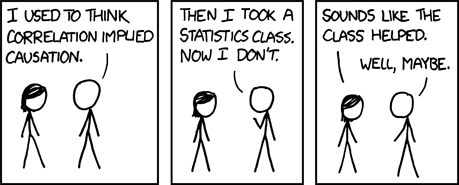
\includegraphics[width=.6\linewidth]{pics/correlation}
\medskip

\url{https://xkcd.com/552/}
}
\end{frame}


\begin{frame}
\frametitle{Continuous random variables 1}
Most interesting data is continuous, i.e.\ $\Vec{x} \in \mathbb{R}^D$: sensor readings, images, \dots

A hack would be to just quantise those data. The explosion of dimensions prohibits this approach---also there is the so-called \emph{curse of dimensionality}.
\begin{itemize}
    \item The distance between two points becomes meaningless in high dimensions (they approach roughly the same value),
    \item Algorithms typically scale super-linear with dimensionality.
\end{itemize}
\medskip

There is really no way around using continuous random variables.
\end{frame}


\begin{frame}
\frametitle{Continuous random variables 2}
Thankfully, many things from the previous slides still hold---with a few changes.
\begin{itemize}
    \item Instead of counting events, we will have to integrate the area of an event (i.e. replace $\sum$ with $\int$),
    \item Consequently, $\int_x p(x) dx = 1$,
    \item The values of a probability function can now exceed $1$,
    \item That is because $p(X=x)$ is meaningless---it has an area of $0$,
    \item We now have to look at intervals, i.e. $p(a < X \leq b)$.
\end{itemize}
\end{frame}


\begin{frame}
\frametitle{Expectation of a random variable}
The expectation of a random variable is a way to summarise its outcome.
It is the value it will take if we average infinitely many outcomes:
\eq{
    \expc[f] = \sum_x f(x) p(x)
}
If we can draw samples from $x$, we can approximate it using $S$ independent samples:
\eq{
    \expc[f] \approx \frac{1}{S} \sum_{s=1}^S f(x_s), x_s \sim X.
}
This is special case of Monte Carlo integration.
\end{frame}


\begin{frame}
\frametitle{Variance of a random variables}
The expectation does not tell us anything about the spread of a random variable.

We might do a gamble if it will earn us \$\,1'000 in expectation. But if it has a chance of 50\% that we will lose \$\,1'000'000 at the same time?

Variance captures this to some extent:
\eq{
    \vari[f] &= \sum_x \bigl(f(x) - \expc[f]\bigr)^2 p(x) \\
        &= \expc\bigl[(f - \expc[f])^2\bigr].
}
It is the expected squared distance from the mean.
\end{frame}



\begin{frame}
\frametitle{Covariance of two random variables}
Often, we want to know how much two variables \emph{vary together}. 
This can be quantified by the \emph{covariance}:
\eq{
    \covari{x}{y} = \expc[xy] - \expc[f]\expc[y].
}
If we look at a multidimensional $\Vec{x}$ with multiple entries, the covariance matrix is defined as:
\eq{
    \covari{\Vec{x}}{\Vec{x}} = \expc[\Vec{x},\Vec{x}^T] - \expc[\Vec{x}]\expc[\Vec{x}]^T.
}
We will get to this again later during linear algebra!
\end{frame}


\begin{frame}
\frametitle{Gaussian distribution}
Most \st{important} convenient distribution for continuous data out there.
\begin{itemize}
    \item Linear combinations of Gaussian random variables are Gaussian.
    \item Sums of sufficiently many independent random variables are Gaussian (aka central limit theorem).
    \item Many important operations can be done in closed form: sampling, evaluation of $p(x)$, conditioning, marginalisation, entropy, \dots
    \item If we know nothing about our data, assuming Gaussianity is the smallest sin we can do.
\end{itemize}


\begin{columns}[t]
\column{5cm}

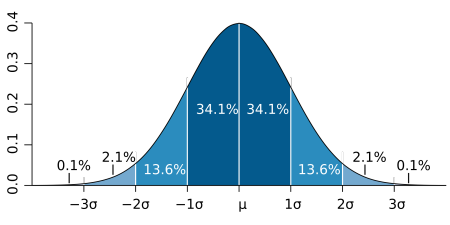
\includegraphics[width=\linewidth]{pics/normal}

\column{5cm}

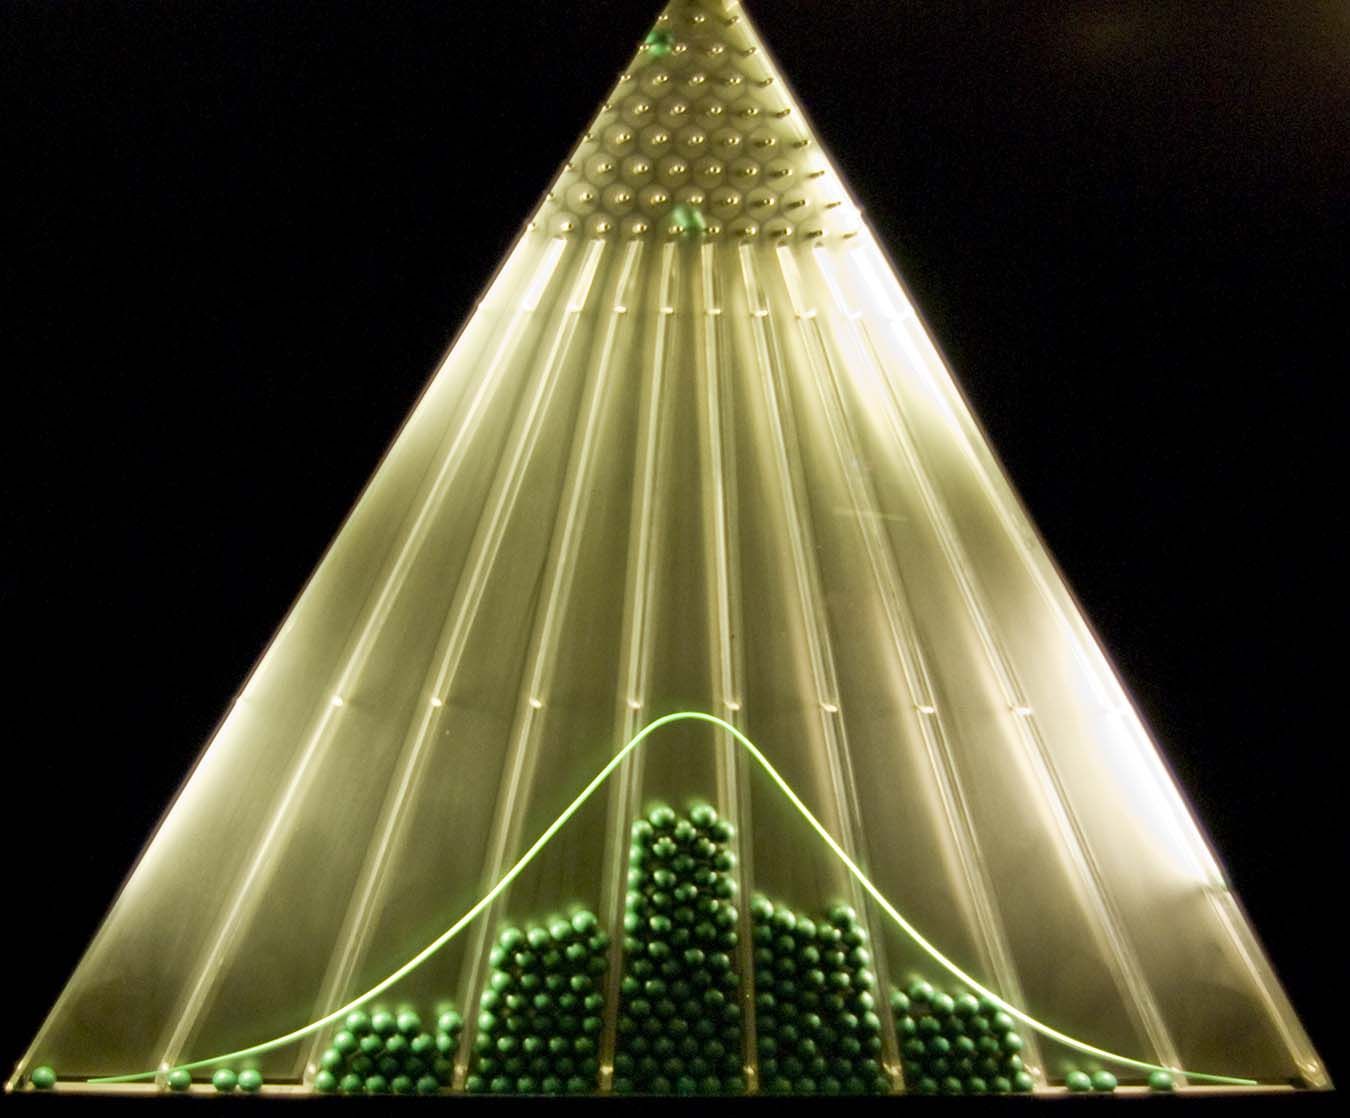
\includegraphics[width=\linewidth]{pics/clt}
\end{columns}


\end{frame}


\begin{frame}
\frametitle{Gaussian distribution 2}
\eq{
    \mathcal{N}(x\mid \mu, \sigma^2) =
        \underbrace{\frac{1}{\sqrt{2\pi\sigma^2}}}_{\text{normalisation}}
        \underbrace{\exp \left [-\frac{(x - \mu)^2}{\sqrt{2\sigma^2}} \right ]}_{\ge 0}
}
The important part is in the exponential---the first part just makes sure that $\int_x \mathcal{N}(x\mid \mu, \sigma^2) dx = 1$.

\end{frame}


\begin{frame}
\frametitle{Maximum Likelihood Estimation 2}
If we observe a couple of random numbers $\mathcal{D} = \{x_i\}_{i=1}^N$, what can we say about their distribution?

We can calculate the mean and the variance. But why?

One way to get there is to assume Gaussianity of the random numbers and identify the parameters $\mu$ and $\sigma^2$ of the distribution using the maximum likelihood principle:
\eq{
    \hat{\mu}, \hat{\sigma}^2 = \argmax_{\mu, \sigma^2} \prod_{i=1}^N \mathcal{N}(x_i\mid \mu, \sigma^2)
}
We maximise the likelihood of the data---i.e. we find the parameters, under which the parameters are the most likely.

\pause
\question{Why the product?}
\pause
\answer{Because we---possibly wrongly---assumed that all $x_i$ are independent of each other.}

\end{frame}

\begin{frame}
\frametitle{Maximum Likelihood Estimation 3}
We will only do the expectation for now.

Logarithm to the rescue. Two important properties:
\begin{itemize}
    \item Logarithm turns products into sums: $\log(\prod x_i) = \sum(\log x_i)$,
    \item Logarithm does not change the location of extrema: $\hat{z} = \argmax_z f(z) \Rightarrow \hat{z} = \argmax_z \log(f(z))$.
\end{itemize}
\end{frame}


\begin{frame}
\frametitle{Maximum Likelihood Estimation 4}
\eq{
    \mathcal{L}(\mu, \sigma^2)
        &= \log \prod_i p(x_i) \\
        &= \sum_i \log \mathcal{N}(x_i\mid \mu, \sigma^2)
}
\pause
Let's look at each of those terms separately.
\eq{
    \log \mathcal{N}(x_i\mid \mu, \sigma^2) 
        &= \log \left [
           \frac{1}{\sqrt{2\pi\sigma^2}}
           \exp \left [-\frac{(x_i - \mu)^2}{\sqrt{2\sigma^2}} \right ] 
           \right ]\\
        &= 
            \underbrace{\log \frac{1}{\sqrt{2\pi\sigma^2}}}_{\text{const wrt }\mu}
           + \cancel{\log \exp} \left [-\frac{(x_i - \mu)^2}{\sqrt{2\sigma^2}} \right ] \\
        &\propto -(x_i - \mu)^2.
}
\pause
Surprise: Fitting a Gaussian is the same as minimising squared error!
\end{frame}


\begin{frame}
\frametitle{Maximum Likelihood Estimation 5}
\eq{
    \mathcal{L}(\mu)
        &= \log \prod_i p(x_i) \\
        &= \sum_i \log \mathcal{N}(x_i|\mu, \sigma^2) \\
        &\propto -\sum_i (x_i - \mu)^2.
}
\pause
Use analysis to find the minimum of this function. Necessary condition:
\eq{
    & \pd{\sum_i -(x_i - \mu)^2}{\mu} = 0 \\
    \Rightarrow& -\sum_i \pd{(x_i - \mu)^2}{\mu} = 0 \\
    \Rightarrow& -\sum_i \cancel{2}x_i - \cancel{2}\mu = 0 \\
    \Rightarrow& \sum_i x_i = N\mu \Rightarrow \mu = \frac{\sum_i x_i}{N}.
}
\end{frame}


\begin{frame}
\frametitle{Summary}
\begin{itemize}
    \item We have seen quite a lot of complicated math today.
    \item It is not necessary to be able to get each detail.
    \item The overall idea is important.
\end{itemize}
\end{frame}


% =====================

\end{document}
